\documentclass{standalone}

\usepackage{tikz}
\usetikzlibrary{arrows.meta, decorations.markings}

\tikzset{
    midarrow/.style={
        decoration={markings, mark=at position 0.5 with {\arrow{Latex}}},
        postaction={decorate}
    }
}

\begin{document}

	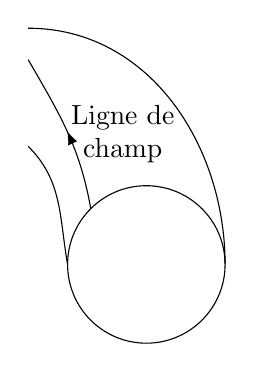
\begin{tikzpicture}
	
	\draw (0,0) circle [radius=1cm];
    
    \draw
    (-1.5,1.5)
    to [out=-45, in=100]
    (-1,0);
    
    \draw
    (-1.5,3)
    to [out=0, in=90]
    (1, 0);
    
    \draw[midarrow]
    (-1.41/2,1.41/2)
    to [out=100, in=-60]
    (-1.5, 2.6);
    
    \node at (-0.3, 1.65) {\shortstack{ Ligne de\\ champ}};
	
	\end{tikzpicture}

\end{document}